\documentclass[12pt,a4paper,openright,twoside]{book}
\usepackage[utf8]{inputenc}
\usepackage{disi-thesis}
\usepackage{code-lstlistings}
\usepackage{notes}
\usepackage{shortcuts}
\usepackage{acronym}

\school{\unibo}
\programme{Corso di Laurea in Ingegneria e Scienze Informatiche}
\title{Utilizzo di Neverlang per la creazione di Domain Specific Languages} %TODO: discuss the title with profs
\author{Terenzi Mirco}
\date{\today}
\subject{Programmazione ad Oggetti}
\supervisor{Prof. Viroli Mirko}
\cosupervisor{Prof. Aguzzi Gianluca}
\session{II}
\academicyear{2023-2024}

% Definition of acronyms
\acrodef{FOP}{Feature Oriented Programming}
\acrodef{DSL}{Domain Specific Language}
\acrodef{JVM}{Java Virtual Machine}
\acrodef{AST}{Abstract Syntax Tree}


\mainlinespacing{1.241} % line spacing in mainmatter, comment to default (1)

\begin{document}

\frontmatter\frontispiece

\begin{abstract}    
Max 2000 characters, strict.
\end{abstract}

%----------------------------------------------------------------------------------------
\tableofcontents   
\listoffigures     % (optional) comment if empty
%\lstlistoflistings % (optional) comment if empty
%----------------------------------------------------------------------------------------

\mainmatter

%----------------------------------------------------------------------------------------
\chapter{Introduzione}
\label{chap:introduzione}
%----------------------------------------------------------------------------------------

Write your intro here.

\paragraph{Struttura della Tesi}

%----------------------------------------------------------------------------------------
\chapter{Background}
\label{chap:background}
%----------------------------------------------------------------------------------------

\section{Domain-Specific Languages}
In modo del tutto opposto rispetto ai linguaggi general-purpose, progettati per poter essere utilizzati in ogni contesto con un’efficienza e 
un grado d’espressività relativamente uguali, i \ac{DSL} sono ottimizzati per uno specifico ambito e risultano essere, in molti casi, una 
soluzione molto più naturale rispetto a quella fornita dai primi \cite{Hudak1997}. Tra gli esempi più comuni di \ac{DSL} troviamo SQL, LaTeX 
(utilizzato anche per la scrittura di questo documento) e CSS.

Nonostante la definizione di \ac{DSL} sia chiara, non è altrettanto immediato definire se un linguaggio sia o meno un \ac{DSL}. In questo caso, 
vi sono alcuni principi chiave da osservare \cite{Fowler2010}:
\begin{itemize}
    \item Un \ac{DSL} è un linguaggio di programmazione e, come tale, la sua struttura dovrebbe essere progettata in modo da essere facile da 
    comprendere per gli esseri umani e, al tempo stesso, eseguibile da un compilatore.
    \item Essendo un linguaggio, deve avere un senso di fluidità e la sua espressività deve essere derivata non solo da un’espressione 
    individuale, ma anche dalla combinazione di più istruzioni.
    \item Coerentemente alla definizione, un \ac{DSL} dovrebbe implementare l'insieme minimo di caratteristiche necessarie per poter supportare 
    il dominio applicativo di interesse ed evitare funzioni non strettamente necessarie che potrebbero rendere il linguaggio più difficile, 
    sia da utilizzare, sia da comprendere.
\end{itemize}

L’utilizzo di questa tipologia di linguaggi di programmazione comporta una serie di vantaggi:
\begin{itemize}
    \item \textbf{Produttività}: È possibile aumentare il livello d’astrazione e, di conseguenza, aumentare la produttività. Questo perché è 
    possibile utilizzare direttamente i concetti propri del dominio applicativo, non essendo limitati dalla necessità di mantenere una 
    generalità atta ad ottenere un linguaggio applicabile in molteplici contesti  \cite{Kelly2008}. Come indicato da Paul Hudak 
    \cite{Hudak1997} ed illustrato nella \cref{fig:sw-dev-cost}, assumendo che il costo di sviluppo di un programma sia lineare, possiamo 
    ipotizzare che il costo iniziale richiesto sia maggiore nel caso si utilizzasse un \ac{DSL} rispetto a metodologie più convenzionali 
    (considerando il caso in cui il linguaggio andasse sviluppato, se ne venisse utilizzato uno esistente tale costo sarebbe significativamente 
    minore). Ciò nonostante, la pendenza della curva è considerevolmente più bassa e quindi, da un determinato punto in poi, l’utilizzo di 
    \ac{DSL} porterebbe un risparmio significativo.
    \begin{figure}
        \centering
        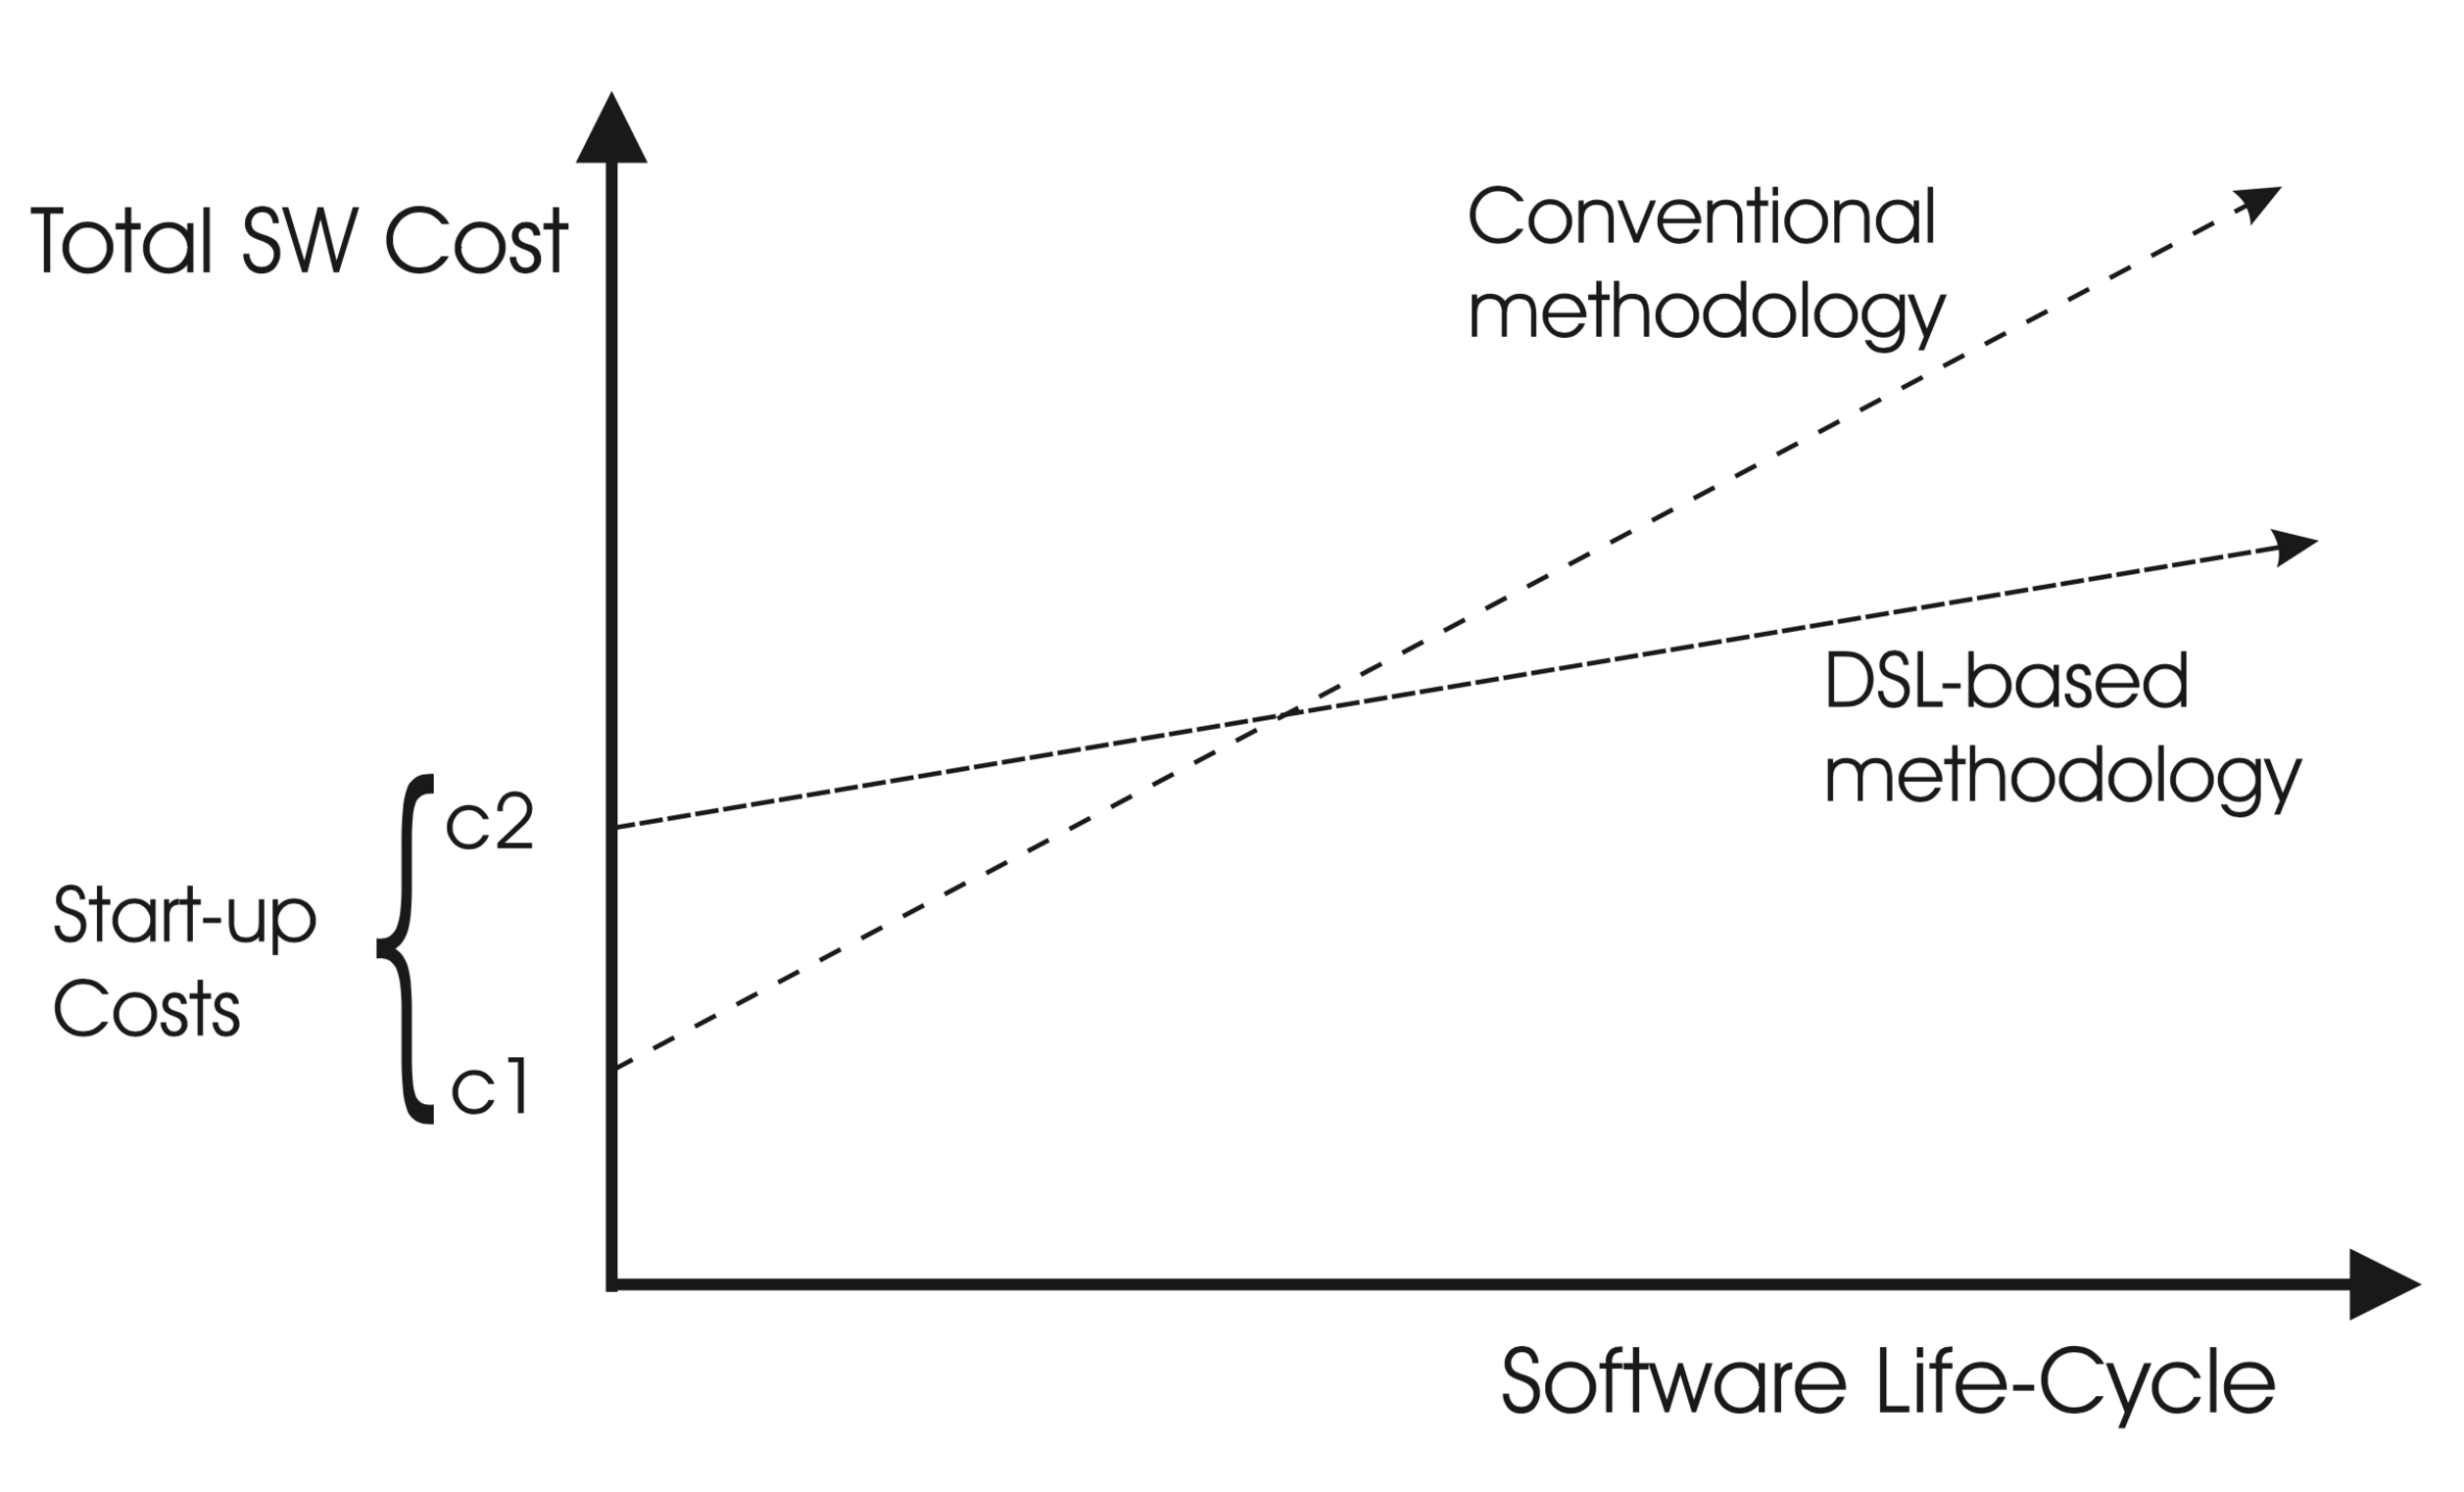
\includegraphics[width=.8\linewidth]{figures/sw-dev-cost.pdf}
        \caption{Il vantaggio ottenuto dall'utilizzo di DSL.}
        \label{fig:sw-dev-cost}
    \end{figure}
    \item \textbf{Qualità del codice}: L'utilizzo di \ac{DSL} favorisce anche una migliore qualità del codice. Infatti, il linguaggio può 
    includere regole direttamente trasposte dal dominio all'interno del quale è applicato. In questo modo risulta molto più difficile, talvolta 
    impossibile, ottenere dei risultati non attesi. Ad esempio, Antti Raunio, capo ingegnere del progetto EADS \cite{EADS}, afferma che ``la 
    qualità del codice generato è chiaramente migliore [...] perché il linguaggio di modellazione è stato progettato per adattarsi 
    all'architettura del nostro terminale''\footnote{Di seguito riportata l'affermazione citata, in lingua originale:``the quality of the 
    generated code is clearly better, simply because the modelling language was designed to fit our terminal architectur''}. Inoltre, 
    l'offuscamento della reale complessità del problema, dovuto all'utilizzo di \ac{DSL}, consente ai nuovi sviluppatori di lavorare ad un 
    alto livello d'astrazione, senza dover conoscere tutti i dettagli inerenti all'implementazione del linguaggio \cite{EADS}. 
    \item \textbf{Migliore manutenibilità}: Sebbene l'uso di \ac{DSL} non renda l'implementazione necessariamente meno complessa di quanto 
    si possa ottenere utilizzando un linguaggio \textit{general-purpose}, la manutenibilità del codice risulta essere accentuata 
    \cite{Klint2010}.  Infatti, considerando il volume del codice, l'utilizzo di \ac{DSL} comporta una minor quantità di codice da comprendere, 
    facilitandone la modifica. Inoltre, è possibile  ignorare il problema di mantenere coerente ciò che è definito dalla grammatica con la 
    struttura gerarchica definita dall'\ac{AST} in quanto quest'ultimo si evolve con la prima \cite{Brabrand2010}.
\end{itemize}

\section{Compilatore}
Il compilatore è un software fondamentale nel campo della programmazione e dell’informatica, il cui compito è tradurre il codice sorgente, 
scritto in un linguaggio di alto livello, in un linguaggio di basso livello, tipicamente il linguaggio macchina o codice oggetto, che può 
essere eseguito 
dal calcolatore.

Il processo di compilazione è suddiviso in diverse fasi, ognuna delle quali ha un ruolo specifico nel convertire il codice sorgente in un 
programma eseguibile. Le fasi principali sono di seguito elencate \cite{Aho2006}:
\begin{itemize}
    \item \textbf{Analisi lessicale}: Durante la fase dell'analisi lessicale, talvolta definita anche \textit{scanning}, la sequenza di 
    caratteri di input viene analizzata e divisa in porzioni significative, chiamate lessemi. Per ogni lessema viene prodotto come output un 
    token, definito come coppia di valori \texttt{<nome-token, valore-attributo>}, che viene processato dalla fase successiva.
    \item \textbf{Analisi sintattica}: La fase dell'analisi sintattica, più comunemente indicata come \textit{parsing} o, in italiano, 
    parsificazione (allo stesso modo, il programma che svolge queste operazioni è chiamato \textit{parser}), prevede che i token siano 
    utilizzati per creare una rappresentazione ad albero che descriva efficacemente la struttura grammaticale dell'input. Un esempio di 
    questo tipo di rappresentazione è costituito dall'albero sintattico. Al suo interno, ogni nodo rappresenta un'operazione e i nodi ad 
    esso discendenti, chiamati anche figli, rappresentano gli operandi dell'operazione definita dal primo. La parsificazione è svolta 
    principalmente secondo due metodologie \cite{Grune2006}:
    \begin{itemize}
        \item l’analisi \textbf{top-down} consiste nell'emulare il processo di produzione della frase. In questo modo, partendo dal simbolo 
        iniziale si procede per fasi ad evolvere l'output in modo da farlo corrispondere alla frase ottenuta come input. Il nome indica che 
        l'albero sintattico viene costruito partendo dall'alto, ossia dal nodo radice, proseguendo verso il basso;
        \item l’analisi \textbf{bottom-up}, al contrario, prevede di invertire il processo di produzione della frase, ossia ha come obiettivo 
        quello di ridurre la frase di input al simbolo iniziale.
    \end{itemize}
    \item \textbf{Analisi semantica}: In questo stadio della compilazione, il fine è analizzare la correttezza semantica del programma. Più 
    nello specifico, vengono utilizzati l'albero sintattico ottenuto dalla fase precedente e la tabella dei simboli per controllare che 
    l'input sia semanticamente coerente con quanto è definito dal linguaggio. Una parte fondamentale dell'analisi semantica è quella del 
    controllo del tipo (in inglese \textit{type-checking}), durante la quale il compilatore si accerta che il valore assegnato ad una 
    variabile sia ammissibile con il tipo di tale variabile e, allo stesso modo, che gli operandi utilizzati in un’operazione siano 
    compatibili con l’operazione stessa. Talora, le specifiche del linguaggio permettono delle conversioni di tipo chiamate coercizioni.
    \item \textbf{Generazione di codice intermedio}: Durante la compilazione, il compilatore genera una o più rappresentazioni intermedie. 
    L'albero sintattico prima descritto rappresenta una delle varie forme che tali rappresentazioni possono assumere. In particolare, devono 
    essere rispettate due proprietà significative: le rappresentazioni devono essere facili da generare e facili da trasporre in codice 
    target (spesso si tratta di linguaggio macchina).
    \item \textbf{Ottimizzazione del codice}: Successivamente, si procede a perfezionare, per quanto possibile, il codice intermedio in modo 
    che si possa poi ottenere un codice finale migliore.
    \item \textbf{Generazione del codice}: Infine, il codice intermedio viene utilizzato per generare il codice target.
\end{itemize}

\section{Neverlang}
Neverlang Language Workbench è un framework sviluppato presso l’Università di Milano dal professor Cazzola e dai suoi collaboratori, il cui 
scopo è favorire lo sviluppo di linguaggi di programmazione, in particolare secondo il paradigma di programmazione feature-oriented.

È basato sull’idea che i linguaggi di programmazione abbiano un’intrinseca divisione modulare in più caratteristiche, o \textit{features}, ciascuna 
delle quali è implementata da un componente specifico. In accordo con tale visione, l’obiettivo del framework è definire i linguaggi tramite 
una divisione in frammenti, chiamati moduli, ognuno dei quali si occupa di implementare una specifica caratteristica e, infine, tramite la 
combinazione dei diversi moduli, ottenere un linguaggio di programmazione specifico per il contesto applicativo richiesto, ossia un  
\ac{DSL} \cite{NeverlangWebsite}.

In particolare, all’interno di ogni modulo vengono definite due parti principali:
\begin{itemize}
    \item la \textbf{sintassi}, utilizzando una grammatica formale;
    \item la \textbf{semantica}, in funzione della sintassi e sfruttando i vari elementi non-terminali e i loro attributi. Inoltre, il 
    comportamento del componente può essere suddiviso in diverse fasi, ciascuna identificata da un ruolo specifico del componente.
\end{itemize}
Successivamente, i componenti del linguaggio vengono definiti combinando definizioni di sintassi e semantica provenienti da diversi moduli, 
all’interno di elementi detti \textit{slice} \cite{Vacchi2015}.

Tra i vantaggi principali di Neverlang troviamo \cite{Cazzola2012}:
\begin{itemize}
    \item \textbf{Modularità}: Ognuno dei moduli che compongono il linguaggio viene compilato separatamente, permettendo di utilizzarne uno o 
    più di uno (in tal caso aggregandoli in uno \textit{slice}) all’interno di altri linguaggi.
    \item \textbf{Riutilizzo}: Neverlang offre la possibilità di riutilizzare frammenti di linguaggio in più di un contesto. Ad esempio, un 
    frammento può utilizzare la sintassi di un altro frammento definito in precedenza e ridefinire la semantica, o viceversa. Inoltre, è 
    possibile ridefinire l’ordine dei simboli non-terminali utilizzati nella sintassi o nella semantica importata.
    \item \textbf{Estensibilità}: L’architettura modulare utilizzata all’interno di Neverlang facilita l’estensione di linguaggi esistenti. 
    Per aggiungere nuove funzionalità non è necessario modificare il codice, ma è sufficiente integrare un nuovo \textit{slice}.
\end{itemize}


\section{Java}
In aggiunta a Neverlang, per la realizzazione del progetto è stato utilizzato il linguaggio di programmazione Java. Java è un linguaggio di 
programmazione ad alto livello, orientato agli oggetti e a tipizzazione statica, sviluppato da Sun Microsystems nel 1991. È molto diffuso e 
ben supportato, con una vasta comunità di sviluppatori e una grande quantità di librerie. Uno degli obiettivi principali di Java è quello di 
essere il più possibile indipendente dalla piattaforma di esecuzione, permettendo di scrivere una volta il codice e farlo eseguire su qualsiasi 
\ac{JVM}, indipendentemente dall'architettura del computer \cite{IBMWebsite}.

Java è stato utilizzato per la realizzazione del progetto in quanto Neverlang è sviluppato per essere completamente integrato con esso.
Il suo compilatore, nlgc, è stato sviluppato per poter convertire il codice scritto utilizzando il DSL di Neverlang, generando un nuovo codice
supportato dalla \ac{JVM}. Inoltre, Neverlang permette di utilizzare Java (ma non solo; anche Scala, ad esempio, è supportato) come linguaggio 
per la definizione della semantica all'interno dei moduli del \ac{DSL}. Ciò è possibile in quanto gli accessi a variabili non-terminali, 
definiti all'interno della sintassi, sono sostituiti dallo specifico plug-in con accessi alla reale rappresentazione interna del linguaggio. 
In particolare, l'accesso alle variabili viene effettuato tramite una chiamata all'n-esimo figlio dell'\ac{AST} \cite{Cazzola2013}.

%----------------------------------------------------------------------------------------
%\chapter{Requisiti}
%\label{chap:requisiti}
%----------------------------------------------------------------------------------------


%----------------------------------------------------------------------------------------
%\chapter{Design e Implementazione}
%\label{chap:Imple}
%----------------------------------------------------------------------------------------


%----------------------------------------------------------------------------------------
%\chapter{Validazione e Conclusioni}
%\label{chap:conclusioni}
%----------------------------------------------------------------------------------------


%----------------------------------------------------------------------------------------
% BIBLIOGRAPHY
%----------------------------------------------------------------------------------------

\backmatter

\bibliographystyle{alpha}
\bibliography{bibliography}

%\begin{acknowledgements} % this is optional
%Optional. Max 1 page.
%\end{acknowledgements}

\end{document}
